%!TEX root = New.tex
\section{The \auspice\ service placement engine}

A key distributed systems challenge in realizing a global name service as described above is the design and implementation of a scalable resolution infrastructure to rapidly resolve identifiers to attributes. To address this challenge, we develop \auspice, a system that automates geo-distributed placement of resolver replicas in a locality and load-aware manner.

\subsection{Design goals and challenges}
\label{sec:design_goals}

An automated resolver replica placement system must satisfy the following design goals.

\begin{enumerate}

\item {\em Low response time}: Replicas of each resolver should be placed close to its end-users so as to minimize user-perceived response times.%\vsp
\item {\em Low update cost}: The number of replicas of each resolver should be controlled so as to limit the update cost required to maintain replica consistency. 
%\vsp
\item {\em Load balance}: The placement of resolver replicas and redirection of client requests should ensure that no single name server location becomes a hotspot.%\vsp
\item {\em Fault-tolerance}: A sufficient number of active or dormant replicas of each resolver must be maintained so as to satisfy its availability objective.
%\vsp
\item {\em Consistency}: The system must achieve the above objectives while respecting the consistency requirements of each resolver.

\end{enumerate}

Although each of the above goals is straightforward and shared by a number of other distributed systems, satisfying the combination of goals is rather challenging. To appreciate why, consider a few straw man alternatives: 

(1) {\em Replicate everything everywhere}: This scheme can minimize response times but can induce a prohibitively high update cost as well as load imbalance. 

(2) {\em Authoritative resolvers(s) plus edge caching}: This scheme maintains one (or a small number of) authoritative resolvers for every name record (similar to today's DNS) and a large number local name servers pull data infrequently from authoritative resolvers. This approach can reduce update bandwidth cost by reusing stale, cached copies of the service's data, however consistency requirements may prevent or severely limit these cost savings, e.g., a mobile host''s name record that is updated frequently may soon become stale requiring a local name server to frequently contact the authoritative resolvers.

%Even for services with weak consistency requirements (e.g., online catalogs), the placement system needs to balance the trade-off between response times and load balance for compute-intensive services.

(2) {\em Consistent hashing with replication}: This approach (e.g., \cite{consistent-hashing}) can ensure load balance and fault-tolerance but may incur high response times as the load balance benefits of randomization are fundamentally at odds with placing resolvers in a locality-aware manner \cite{codons,cox, beehive}. Significantly increasing the number of resolvers  can improve response times but also increase update cost for write-intensive services.

In accordance with our design goals, Auspice explicitly determines the number and placement of resolver replicas for an identifier taking into account its query and update rates and the geographic locality of queries, and redirects client requests taking into account the aggregate load at each name server. We describe this design in detail in section TBD.


\begin{figure}[t]
\centering
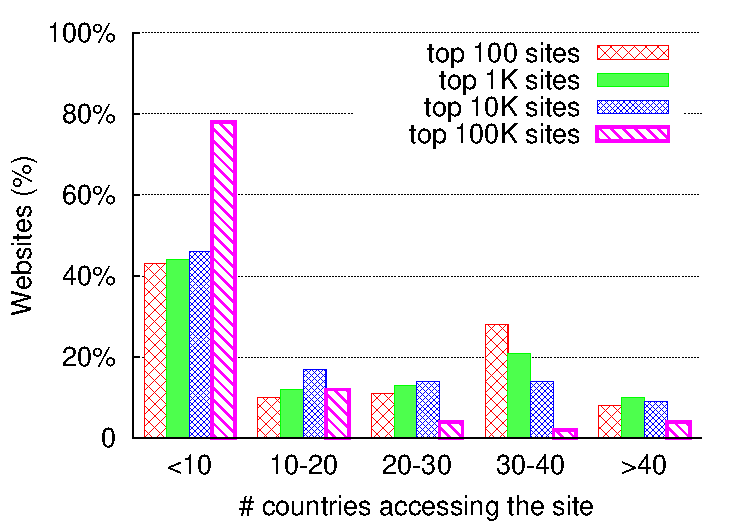
\includegraphics[scale=0.6]{figure/numcountry_boxplot.pdf}
\vspace{-0.1in}
\caption{Locality in website popularity: 40\% websites are accessed in less than 10 countries.}
\label{fig:localityweb}
\end{figure}


\subsection{Geographic locality}

%Replicating name records in locality-aware manner minimizes request latencies as well as update costs. 
If request patterns show geo-locality, placing a small number of resolvers in a locality-aware manner achieves low request latencies; the cost of keeping resolvers updated is minimized by creating a small number of resolvers. Our analysis of of geo-distribution of today's websites' traffic suggests that request patterns for their name records  show a high degree of geo-locality\tbd{Do you have a breakdown by grids of fixed size? Countries can vary greatly in size. Also, are google and facebook accessed in just 40 countries? This seems very likely wrong.}. We argue that name records for mobile hosts are likely to show even stronger geo-locality patterns, thereby making the case for a locality-aware placement of resolvers\tbd{On what basis are you arguing? Do you have a reference or a justification?}.

%Our design is motivated in part by two key features of the workload that the naming service is expected to handle: high update rates of name records, and geo-locality of distribution of requests.  A mobile host rapidly changes the set of networks it is connected to and thus requires frequent updates to its name record. 
 
\begin{table}[t]
\centering
\begin{tabular}{ l | c | c}
\hline
rank \& site & \# countries & country most accessed\\
  & accessing  & \& traffic percentage\\
\hline
\hline
1, google.com & 36 & US \ 37.3\% \\ 
\hline
2, facebook.com & 40 & US \ 19.6\% \\
\hline
3, youtube.com & 39 & US \ 19.1\% \\
\hline
4, yahoo.com & 31 & US \ 32.8\% \\
\hline
\rowcolor[gray]{0.9} 5, baidu.com & 5 & CN \ 96.8\% \\
\hline
6, wikipedia.org & 34 & US \ 19.9\% \\
\hline
7, live.com & 33 & US \ 15.3\%\\
\hline
\rowcolor[gray]{0.9} 8, amazon.com & 19 & US \ 74.9\%\\
\hline
\rowcolor[gray]{0.9} 9, qq.com & 5 & CN \ 95.5\%\\
\hline
10, twitter.com & 31 & US \ 26.4\%\\
 \hline
\end{tabular}
\caption{Locality in top 10 sites: two sites baidu.com and qq.com have 95\% traffic coming from a single country.}
\label{tab:top10web}
\end{table}

 
We analyze geo-locality of today's websites using Alexa TopSites dataset  \cite{alexa}, which provides ranking of today's top websites, and geo-distribution  of  each website's requests. These statistics are based on page views for each website, but we expect the number of name record requests for a website to be proportional  (or positively correlated) to its page views in a geographic region. 


Figure \ref{fig:localityweb} shows the geo-locality in website popularity: it plots the percentage of websites that are accessed in different numbers of countries. 40\% websites are accessed in less than 10 countries for the top 100, 1K, 10K sites and the percentage value goes up to 80\% for the top 100K sites.  Table \ref{tab:top10web} further zooms into the access statistics for the top 10 popular websites. Geo-locality persists in the top 10 sites and is prominent for three sites: baidu.com and qq.com which have 95\% traffic coming from a single country China and amazon.com which has 75\% traffic coming from United States.
Thus, a locality-aware placement of resolvers is a natural choice, e.g., China for baidu.com and qq.com and US for amazon.com.

The name record of a mobile host (\emph{mobile name} for short) is likely to show a strong geo-locality of requests. This is due to several reasons.
Updates for mobile names will originate from the mobile host itself, whose mobility will be contained in a small geographic region for most hosts.
Lookups for a mobile name will be done by web services to push updates to the mobile host. Today's web services are geo-replicated to position themselves closer to end-users. Most likely, the closest service replica will lookup for the mobile name, giving rise to geo-locality.
Another source of a mobile name's queries is communication between two mobile hosts, e.g., a user's friends contacting the user's mobile device to send messages.
We expect these queries to come from a user's contacts list. Since most of a user's contacts are expected to be within  the same country, these  queries will exhibit strong geo-locality patterns as well.


\eat{
\subsection{Geo-distributed cloud services}
Geo-distributed computing clouds today offer a scalable and cost-effective solution for hosting a variety of online services such as search, social networking, web portals, e-commerce, etc. These clouds are typically hosted by a large hosting service provider that is responsible for allocating resources on demand to a large number of hosted enterprise services. Examples of such hosting environments include Amazon's AWS suite \cite{amazonec2}, Google's AppEngine \cite{google-app-engine}, Akamai's Edge Computing \cite{edgecomputing}, and Windows Azure \cite{windowsazure}. The hosted services benefit from economies of scale, agile provisioning of on-demand resources, and ease of management that comes with cloud hosting. Geo-distributed clouds are particularly attractive as they enable hosted services to locate themselves close to their end-users, thereby significantly improving user-perceived latency.

To appreciate it, we performed a large scale case study on two cloud-based services --- naming service for Alexa TopSites and online social networking service for Twitter users. Alexa TopSites \cite{alexa} provides lists of web sites ranked by their worldwide traffic statistics. Each website relies on a naming service to direct requests to appropriate name resolvers.
Users of Twitter \cite{twitter} depends on the underlying social networking service infrastructure to deliver status updates that they share ideas, activities and events with their friends. 
A more detailed description of how we collect data from these services is deferred to section \ref{sec:eval}. Our explored study based on 100,000 Alexa websites and TBD Twitter users reveal strong localities in user access pattern, a feature that can benefit significantly by agile service placement.

Figure \ref{fig:localityweb} shows the locality in website popularity: it plots the percentage of websites that are accessed in different numbers of countries. 40\% websites are accessed in less than 10 countries for the top 100, 1K, 10K sites and the percentage value goes up to 80\% for the top 100K sites. 
Table \ref{tab:top10web} further zooms into the access statistics for the top 10 popular websites. The first and second columns show the rank, name and number of countries that access a site, and the third column shows the country that accesses the site most and its corresponding traffic percentage. Locality persist in the top 10 sites and is prominent for three sites: baidu.com and qq.com which have 95\% traffic coming from a single country China and amazon.com which has 75\% traffic coming from United States.
Thus, it is natural for a website naming service to place resolver replicas close to pockets of demand, e.g., China for baidu.com and qq.com and US for amazon.com.

However, a critical limitation of geo-distributed clouds today is that each hosted service has to manually determine the geographic locations of replicas of their service. Hosted services typically select these locations by monitoring the geolocations of end-user requests at coarse-grained timescales (e.g., several weeks or months) and creating new replicas or migrating existing ones close to regions of heavy demand. Furthermore, as each hosted service determines its replica locations independently, the hosting service provider may experience hotspots at one or more locations resulting in SLA violations and revenue loss.

Our position is that service replica placement for hosted services can and should be automated by hosting service providers. Automated placement obviates redundant effort on part of hosted services and enables the hosting service provider to manage its global resources in a more efficient and agile manner.
}


% related to service placement.
\eat{
Clearly, it is not easy to design a general-purpose placement engine that can satisfy all of the above goals for arbitrary services. So, we restrict the scope of this paper to services with a single bottleneck resource. This restriction allows us to measure the demand for each service and the available capacity at each hosting site with a scalar metric, e.g., the demand for each service and the aggregate capacity at a site can be measured in requests/sec. Note that this restriction does not imply that the services or requests have to be homogeneous, only that their aggregate demand can be specified as a scalar. For example, suppose service A  is a web server with a demand of 250 requests/sec and the maximum sustainable throughput for service A (in isolation) at the site is 1000 requests/sec, and service B is a database server with a demand of 80 queries/sec with a corresponding maximum sustainable throughput of 400 queries/sec. Further suppose that both services are bottlenecked by a single resource, e.g. they are both compute-bottlenecked or they are both IO-bottlenecked or they are both bandwidth-bottlenecked. In this example, it is straightforward to see that the site has enough capacity to place both services as service A uses 25\% of the capacity and service B uses 20\% of the capacity.

Although the above assumption allows us to accommodate a large class of services and hosting scenarios, it does limit the types of supportable services. For example, suppose service A is memory-bottlenecked and has a demand corresponding to 75\% of the maximum throughput sustainable for A alone at that location, and service B is network-bandwidth-bottlenecked with a demand corresponding to 80\% of the maximum sustainable throughput for B alone. Without additional information about each service, it is not possible to determine if both A and B can be placed at the location. More importantly, even if one could measure the usage of each resource for each service, the distributed nature of the problem makes load balancing in scenarios with such ``multi-dimensional'' resource constraints much harder. As a result, the problem of automatically placing arbitrary services (and in particular virtual machines running ``black-box'' services) is not within the scope of \auspice's design.
}

\eat{
% why DNS will not work.
A global  name resolution service for mobile hosts requires a radically different design than the current DNS, which caters to immobile hosts whose network addresses are updated infrequently. 
The current DNS design manages to provide an acceptable performance due to heavy reliance on TTL-based caching.
Name records for mobile hosts would be updated at orders of magnitude higher rates than name records in today's  DNS. For example, a mobile host may change network addresses tens of times per day, while a domain name's IP address does not change for weeks or even months.
A high update rate of name records dictates that TTL values are set to orders of magnitude shorter values, e.g. few seconds instead of 6 hours or one day. In the current DNS design, short TTLs will cause requests for name records of mobile hosts to frequently contact a small number of authoritative name servers for that name record, resulting in very high latencies.

% replicate-all high costs
An obvious solution to improve performance is to replicate every name record at a large number of locations around the globe. However, maintaining the consistency of a large number of name record resolvers increases the update cost,  both in terms of network bandwidth and server resources.
The update cost would be manageable if the name record is updated infrequently such as  the current DNS's  name records.
The update costs for billions of mobile devices, updating addresses up to 100 times per day,  would require processing a million updates per second at every location.
Clearly, a ``replicate everywhere'' strategy would, at best, add substantial costs to the service, or might even be infeasible. 

% intuition behind our design
This leads us to ask if we can design a replication strategy with much smaller cost of updates that yet achieves small response latency. As the update cost increase with the  rate at which a name record is updated, this suggests that the number of resolvers of a name record should be inversely proportional to its update rate. By this thumb rule, the name  record of a mobile host has a high update rate and therefore must be replicated at a small number of locations.

To provide low response latencies with a small number of resolvers, resolvers must be located close to the pockets of demand. This rules out designs that augment consistent hashing with a small amount of replication \cite{codons,cox, beehive}. These designs can ensure load balance and fault-tolerance but may incur high response times as the load balance benefits of randomization are fundamentally at odds with placing resolvers in a locality-aware manner. In this paper, we propose an approach that explicitly measures the geo-distribution of  requests and replicates name records in a locality and load-aware manner. This results in an order-of-magnitude lower update costs than a replicate everywhere scheme, and yet achieves close to the best response latencies.
 }